\documentclass[titlepage,a4paper,12pt]{ltjsreport}

\usepackage{luatexja}
\usepackage{amsmath,amsfonts}
\usepackage{amsthm}
\usepackage{bm}
\usepackage[dvipdfmx]{graphicx}
\usepackage{color}
\usepackage{caption}
\usepackage{url}
\usepackage{listings}
\usepackage{abstract}
\usepackage{multicol}
\usepackage{geometry}
\usepackage{here}

\lstset{
    basicstyle={\ttfamily},
    identifierstyle={\small},
    commentstyle={\small},
    keywordstyle={\small\bfseries},
    ndkeywordstyle={\small},
    stringstyle={\small\ttfamily},
    frame={tb},
    breaklines=true,
    columns=fixed,
    basewidth=0.465em,
    numbers=left,
    numberstyle={\scriptsize},
    lineskip=-0.5ex
}


\begin{document}

\leftline{課題1 要求記述}
\rightline{256E0143
三留 慎太郎}

\begin{enumerate}
    \item 概要 \mbox{}\\
    $n$個のデータ対の集合に対して線形回帰パラメータ$\beta_0, \beta_1,$ 相関係数$r_{x,y}, r^2$を計算する。\\
    与えられた見積もり値$x_k$に対して,$y_k = \beta_0 + \beta_1x_k$を満たす予測値$y_k$を計算する

    \item 詳細\mbox{}\\
    回帰パラメーター$\beta_1,\beta_0$は$x,y$の平均$x_{avg},y_{avg}$を用いて以下の式で求められる。
    \[\beta_1 = \frac{(\sum_{i=1}^{n}x_iy_i) - (nx_{avg}y_{avg})}{(\sum_{i=1}^{n}x_i^2) - (nx_{avg}^2)}\]
    \[\beta_0 = y_{avg} - \beta_1x_{avg}\]

    相関係数$r_{x,y}, r^2$は以下の式で求められる
    \[
    r_{x,y} = \frac{n (\sum_{i=1}^{n} x_i y_i) - (\sum_{i=1}^{n} x_i) (\sum_{i=1}^{n} y_i)}
    {\sqrt{\left[n \sum_{i=1}^{n} x_i^2 - (\sum_{i=1}^{n} x_i)^2\right]
    \left[n \sum_{i=1}^{n} y_i^2 - (\sum_{i=1}^{n} y_i)^2\right]}}
    \]

    \[r^2 = r_{x,y}^2\]

    しかし、相関係数$r_{x,y}$は$x,y$の標準偏差$\sigma_x,\sigma_y$を用いての以下の式に変換できるため、それを利用して以下で求める。

    \[r_{x,y} = \beta_1\frac{\sigma_x}{\sigma_y}\]

    
    ここで$n$は与えられるデータ対の数、$x_i$は$i$個目の実数の値を表す。\\
    また、与えられる$n$個のデータ対は、双方向リンクリストを用いて操作する。


    \item 入力\mbox{}\\
    
    \begin{itemize}
        \item データの入力:csvファイル入力
        \item 入力ファイル:ファイル例の図\ref{datapair}のように、カンマ区切りの表形式で表現し、同じ列に同じ属性のデータを格納する。\\
        
        なお,与えるデータの各列は以下のデータを表す.
        \begin{itemize}
            \item 1列:代替品の規模見積もり
            \item 2列:追加修正の計画規模
            \item 3列:追加修正の実績規模
            \item 4列:実績開発時間
        \end{itemize}
        
        \begin{figure}[H]
            \centering
            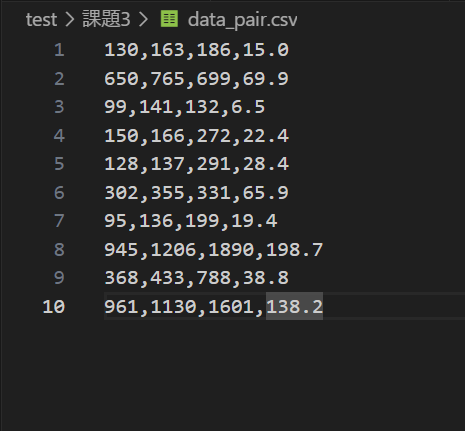
\includegraphics[width=0.4\textwidth]{../picture/課題3/datapair.png}
            \caption{データ対入力ファイル例}
            \label{datapair}
        \end{figure}
        
        \item 実行時の入力:コマンドラインに以下の形式で入力
         java プログラム名 実数値入力ファイル名 $x$として用いる列の番号 $y$として用いる列の番号 $x_k$
        \item 実行時入力例:java Program3 data\_pair.csv 2 3 386\\
                

    \end{itemize}


    \item 出力\mbox{}\\
    \begin{itemize}
        \item 出力方法:コマンドライン出力
        \item 出力する値:回帰パラメータ$\beta_0,\beta_1$、相関係数$r_{x,y},r^2$、予測値$y_k$
        \item 精度:必要に応じて少数第7位を四捨五入して表示する。
        \item 出力例:図\ref{outexample}のように出力する値をそれぞれb\_0, b\_1, r\_xy, r\^2, y\_kとして改行して表示する。
        
        \begin{figure}[H]
            \centering
            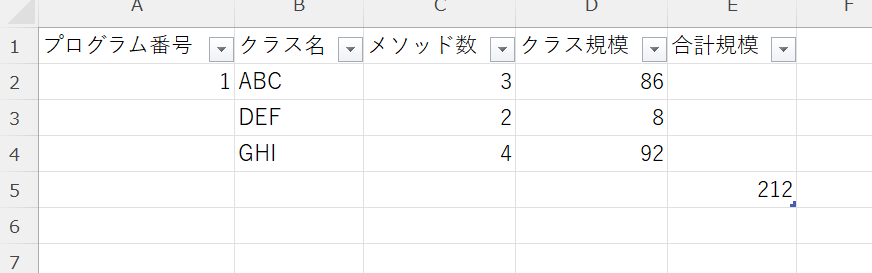
\includegraphics[width=0.4\textwidth]{../picture/課題3/out_example.png}
            \caption{出力例}
            \label{outexample}
        \end{figure}

    \end{itemize}


    \item テスト\mbox{}\\
    図\ref{datapair}のデータをもちいて、$x,y$を以下の4つ組み合わせでテストを行い、それぞれの期待値を図\ref{kitaichi1},図\ref{kitaichi2},図\ref{kitaichi3},図\ref{kitaichi4}に示す。\\
    ただし,代理品の規模見積もりは$x_k$=386として与えられている.

    \begin{itemize}
        \item テスト1:$x$:代理品の規模見積もり、$y$:追加修正の実績規模
        \item テスト2:$x$:代理品の規模見積もり、$y$:実績開発時間
        \item テスト3:$x$:追加修正の計画規模、$y$:追加修正の実績規模
        \item テスト4:$x$:代理品の規模見積もり、$y$:追加修正の実績規模
    \end{itemize}

    \begin{figure}[h]
        \centering
        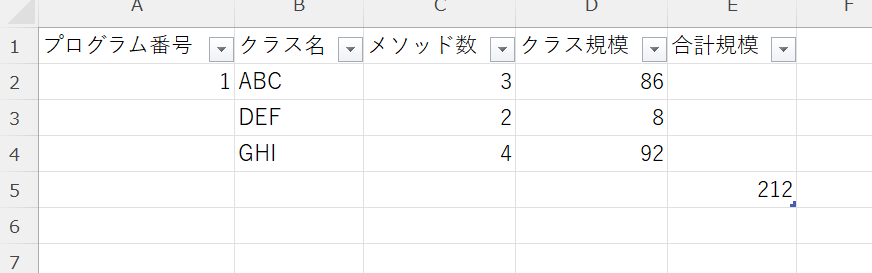
\includegraphics[width=0.4\textwidth]{../picture/課題3/out_example.png}
        \caption{期待値1}
        \label{kitaichi1}
    \end{figure}
    
    \begin{figure}[h]
        \centering
        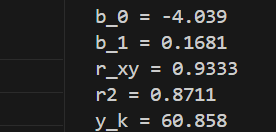
\includegraphics[width=0.4\textwidth]{../picture/課題3/kitaichi2.png}
        \caption{期待値2}
        \label{kitaichi2}
    \end{figure}

    \begin{figure}[h]
        \centering
        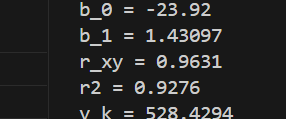
\includegraphics[width=0.4\textwidth]{../picture/課題3/kitaichi3.png}
        \caption{期待値3}
        \label{kitaichi3}
    \end{figure}
    
    \begin{figure}[h]
        \centering
        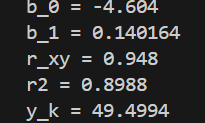
\includegraphics[width=0.4\textwidth]{../picture/課題3/kitaichi4.png}
        \caption{期待値4}
        \label{kitaichi4}
    \end{figure}
    
    
     

\end{enumerate}



\end{document}